\documentclass[tikz,border=5pt]{standalone}
\usepackage{tikz}

\begin{document}

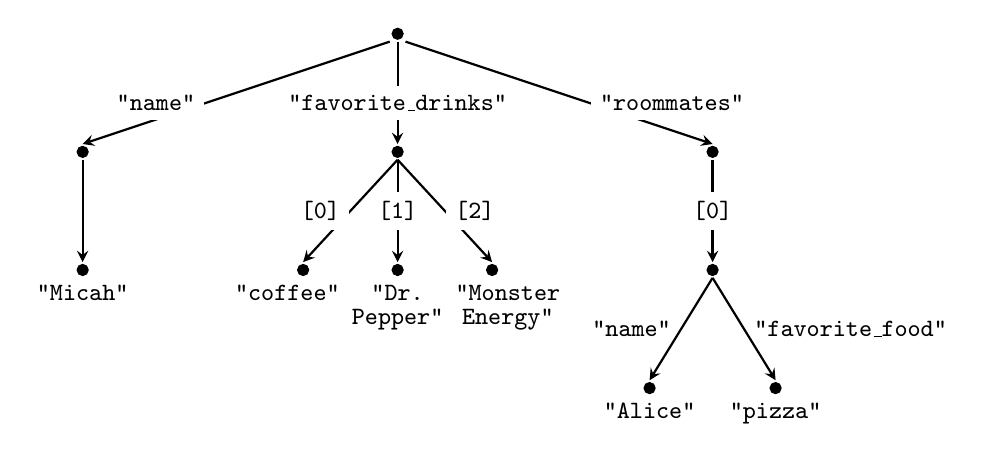
\begin{tikzpicture}[>=stealth]

% nodes
\filldraw (0,0) circle (2pt)

(-4,-1.5) circle (2pt)
(0,-1.5) circle (2pt)
(4,-1.5) circle (2pt)

(-4,-3) circle (2pt)

(-1.2,-3) circle (2pt)
(0,-3) circle (2pt)
(1.2,-3) circle (2pt)

(4,-3) circle (2pt)

(3.2,-4.5) circle (2pt)
(4.8,-4.5) circle (2pt)
;

% edges root -> keys
\path (-0.1,-0.1) edge[->, thick] node[pos=0.6,left,fill=white] {\small \texttt{"name"}} (-4,-1.4);
\path (0,-0.1) edge[->, thick] node[pos=0.6,fill=white] {\small \texttt{"favorite\_drinks"}} (0,-1.4);
\path (0.1,-0.1) edge[->, thick] node[pos=0.6,right,fill=white] {\small \texttt{"roommates"}} (4,-1.4);

% name value
\path (-4,-1.6) edge[->, thick] node[pos=0.5,left] {} (-4,-2.9);

% favorite_drinks array
\path (0,-1.6) edge[->, thick] node[pos=0.5,left,fill=white] {\small \texttt{[0]}} (-1.2,-2.9);
\path (0,-1.6) edge[->, thick] node[pos=0.5,fill=white] {\small \texttt{[1]}} (0,-2.9);
\path (0,-1.6) edge[->, thick] node[pos=0.5,right,fill=white] {\small \texttt{[2]}} (1.2,-2.9);

% roommates array
\path (4,-1.6) edge[->, thick] node[pos=0.5,align=center,fill=white] {\small \texttt{[0]}} (4,-2.9);

% roommate object fields
\path (4,-3.1) edge[->, thick] node[pos=0.5,left] {\small \texttt{"name"}} (3.2,-4.4);
\path (4,-3.1) edge[->, thick] node[pos=0.5,right] {\small \texttt{"favorite\_food"}} (4.8,-4.4);

% value labels
\draw (-4,-3) node[below=2pt] {\small \texttt{"Micah"}};

\draw (-1.4,-3) node[below=2pt] {\small \texttt{"coffee"}};
\draw (0,-3) node[below=2pt] {\small \texttt{\shortstack{"Dr.\\Pepper"}}};
\draw (1.4,-3) node[below=2pt] {\small \texttt{\shortstack{"Monster\\Energy"}}};

\draw (3.2,-4.5) node[below=2pt] {\small \texttt{"Alice"}};
\draw (4.8,-4.5) node[below=2pt] {\small \texttt{"pizza"}};

\end{tikzpicture}

\end{document}
